% Provenance (never printed): cycle 4 SVT, "La planete Terre, l'environnement
% et l'action humaine": natural risks, hazard and vulnerability, prevention
% and protection; see sources/book1/PROVENANCE.md. Book 1, grade 9, chapter 2.
% Vocabulary guard: owns risk, vulnerability, prevention, hazard map.
% Natural hazard and natural disaster, the warning colours and the safety
% rules are g5's (natural-hazards); the warning signs of an eruption and the
% Pinatubo story are g7's (volcanoes); seismometer, tsunami and "scientists
% cannot predict earthquakes" are g7's (earthquakes); flood and floodplain
% are g5's (water-shapes-the-land); weather forecast is g8's. Lahars are
% called mudflows (as in g7). "Normal fault" is Book 2's: here "a fault".
\chapter{Vivir con los riesgos naturales}\label{ch:g9:natural-risks}

A última hora de la tarde del 13~de noviembre de 1985, la mayoría de los
habitantes de Armero, una ciudad de Colombia, estaban acostados. Una
\omterm{def:g5:natural-hazards:storm}{tormenta} ocultaba el \omterm{def:g4:volcanoes-earthquakes-first-look:volcano}{volcán} Nevado del Ruiz, a \qty{45}{km}, y nadie en la
ciudad lo vio entrar en \omterm{def:g4:volcanoes-earthquakes-first-look:eruption}{erupción}. Las \omterm{def:g3:stones-pebbles-sand:rock}{rocas} calientes fundieron parte de su
hielo, y el agua, mezclada con ceniza y \omterm{def:g3:stones-pebbles-sand:rock}{rocas}, bajó a toda velocidad por
los \omterm{def:g1:landscapes-around-us:landform}{valles} en forma de coladas de \omterm{def:g3:stones-pebbles-sand:sand}{barro}. Unas dos horas después, las
coladas salieron del \omterm{def:g1:landscapes-around-us:landform}{valle} del \omterm{def:g1:landscapes-around-us:water}{río} Lagunillas y entraron directamente en
la ciudad: murieron unas \num{23000} personas, la mayor parte de la
población. Dos horas eran tiempo suficiente para llegar a pie a un terreno
más alto. A los habitantes de Armero no se les avisó.
% ledger: usgs:armero

\begin{omfigure}
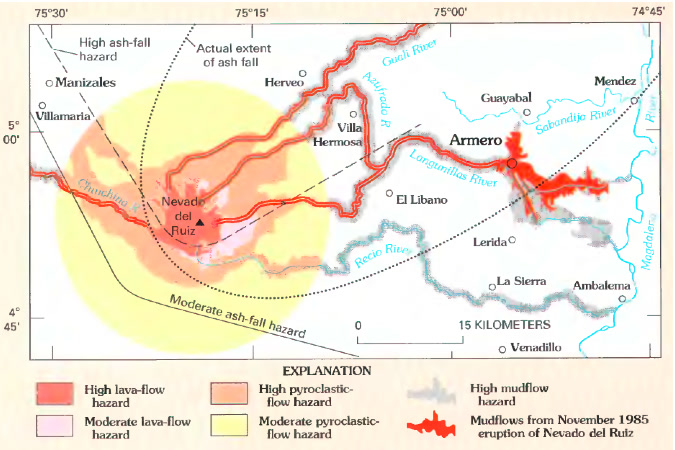
\includegraphics[width=0.86\linewidth]{images/book1/g9-ruiz-hazard-map.jpg}

{\small El \omterm{def:g9:natural-risks:hazard-map}{mapa de peligrosidad} del Nevado del Ruiz. Una primera versión,
elaborada por geólogos colombianos, circuló un mes antes de la \omterm{def:g4:volcanoes-earthquakes-first-look:eruption}{erupción} y
ya mostraba el peligro de coladas de \omterm{def:g3:stones-pebbles-sand:sand}{barro} en el \omterm{def:g1:landscapes-around-us:landform}{valle} de Armero. Esta
versión, redibujada después de la catástrofe, añade en rojo vivo las
coladas de \omterm{def:g3:stones-pebbles-sand:sand}{barro} que llegaron realmente en noviembre de 1985 (el círculo
sombreado alrededor del \omterm{def:g4:volcanoes-earthquakes-first-look:volcano}{volcán} tiene un radio de unos \qty{20}{km}). Según
T.~L.~Wright y T.~C.~Pierson, USGS Circular 1073, 1992 (dominio público, vía
Wikimedia Commons).}
% ledger: usgs:ruiz-map, commons:ruiz-map
\label{fig:g9:natural-risks:ruiz}
\end{omfigure}

Seis años después, en el monte Pinatubo, en Filipinas, el \omterm{def:g4:volcanoes-earthquakes-first-look:volcano}{volcán} estaba
vigilado, la alerta llegó a tiempo y la población se marchó
(\cref{ch:g7:volcanoes}). Los dos eran \omterm{def:g4:volcanoes-earthquakes-first-look:volcano}{volcanes} explosivos, con gente
viviendo en el camino de sus coladas de \omterm{def:g3:stones-pebbles-sand:sand}{barro}. Lo que cambiaba era lo que
sabía la gente y lo que hizo con ello. Este capítulo trata de esa
diferencia.
% ledger: usgs:armero (Pinatubo 1991 averted a disaster like Armero), usgs:pinatubo-1991

\begin{recall}
Un \emph{\omterm{def:g5:natural-hazards:hazard}{peligro natural}} es un fenómeno natural que puede causar daños a
las personas; se convierte en una \emph{\omterm{def:g5:natural-hazards:disaster}{catástrofe natural}} cuando golpea
donde vive gente y causa grandes daños (\cref{ch:g5:natural-hazards}). Un
\omterm{def:g1:landscapes-around-us:water}{río} que se desborda cubre su \omterm{def:g5:water-shapes-the-land:flood}{llanura de inundación}
(\cref{ch:g5:water-shapes-the-land}). Un \omterm{def:g4:volcanoes-earthquakes-first-look:volcano}{volcán} suele dar señales de alerta
antes de una gran \omterm{def:g4:volcanoes-earthquakes-first-look:eruption}{erupción}: pequeños \omterm{def:g4:volcanoes-earthquakes-first-look:earthquake}{terremotos}, laderas que se hinchan,
gases (\cref{ch:g7:volcanoes}). Los científicos no pueden predecir los
\omterm{def:g4:volcanoes-earthquakes-first-look:earthquake}{terremotos}; los \omterm{def:g7:earthquakes:seismometer}{sismómetros} los registran, y un \omterm{def:g4:volcanoes-earthquakes-first-look:earthquake}{terremoto} bajo el \omterm{def:g2:water-on-earth:ocean}{mar}
puede desencadenar un \omterm{def:g7:earthquakes:tsunami}{tsunami} (\cref{ch:g7:earthquakes}). Una \omterm{def:g8:fronts-and-weather-maps:forecast}{previsión
meteorológica} dice qué \omterm{def:g1:watching-the-weather:weather}{tiempo} hará en los próximos días
(\cref{ch:g8:fronts-and-weather-maps}).
\end{recall}

\section{Peligro, vulnerabilidad y riesgo}

El mismo \omterm{def:g4:volcanoes-earthquakes-first-look:earthquake}{terremoto} no causa los mismos daños en todas partes. Bajo un
\omterm{def:g5:weather-and-climate:desert}{desierto} vacío no daña a nadie. Bajo una ciudad de edificios sólidos cuyos
habitantes saben qué hacer, sacude, asusta y rompe cristales. Bajo una
ciudad de casas pesadas y mal construidas, puede derrumbarlas sobre la
gente que hay dentro. El peligro es el mismo; lo que cambia es la
facilidad con que el lugar puede sufrir daños.

\begin{definition}[Vulnerabilidad]\label{def:g9:natural-risks:vulnerability}
La \emph{vulnerabilidad}\index{vulnerabilidad} de un lugar es la facilidad
con que sus habitantes, sus edificios y las cosas que necesitan pueden
sufrir daños por un \omterm{def:g5:natural-hazards:hazard}{peligro natural}. Las viviendas en una \omterm{def:g5:water-shapes-the-land:flood}{llanura de
inundación}, los edificios débiles, la falta de alerta y la falta de plan
hacen vulnerable un lugar.
\end{definition}

\begin{definition}[Riesgo]\label{def:g9:natural-risks:risk}
El \emph{riesgo}\index{riesgo} al que se enfrenta un lugar ante un \omterm{def:g5:natural-hazards:hazard}{peligro
natural} es la amenaza de daños para sus habitantes y sus bienes. Depende a
la vez del peligro, de su intensidad y su frecuencia, y de la
\omterm{def:g9:natural-risks:vulnerability}{vulnerabilidad} del lugar: donde no hay peligro, o no hay nada que pueda
sufrir daños, no hay riesgo.
\end{definition}

\begin{omfigure}
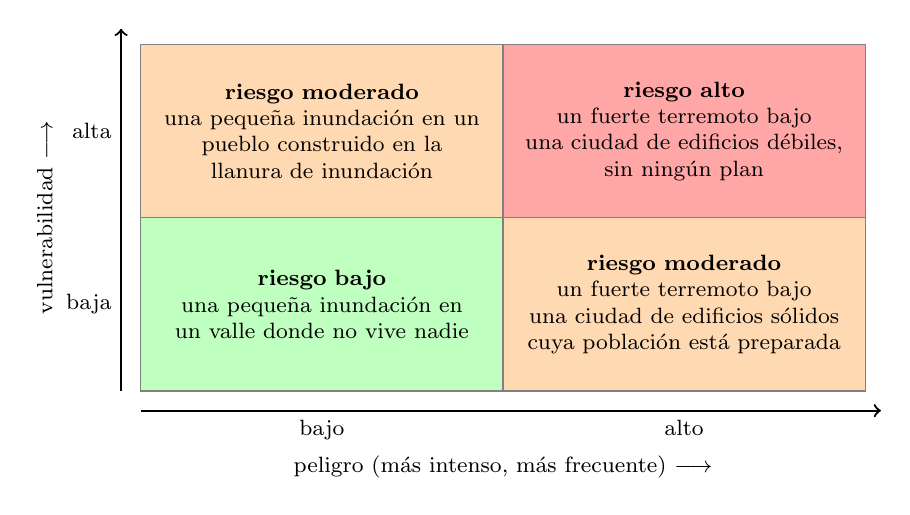
\begin{tikzpicture}[x=1cm, y=1cm, font=\footnotesize,
    cell/.style={minimum width=4.6cm, minimum height=2.2cm, align=center, draw=black!50, text width=4.2cm}]
  \node[cell, fill=green!25] at (2.3,1.1) {\textbf{riesgo bajo}\\ una pequeña inundación en\\ un valle donde no vive nadie};
  \node[cell, fill=orange!30] at (6.9,1.1) {\textbf{riesgo moderado}\\ un fuerte terremoto bajo\\ una ciudad de edificios sólidos\\ cuya población está preparada};
  \node[cell, fill=orange!30] at (2.3,3.3) {\textbf{riesgo moderado}\\ una pequeña inundación en un\\ pueblo construido en la\\ llanura de inundación};
  \node[cell, fill=red!35] at (6.9,3.3) {\textbf{riesgo alto}\\ un fuerte terremoto bajo\\ una ciudad de edificios débiles,\\ sin ningún plan};
  \draw[->, thick] (0,-0.25) -- (9.4,-0.25);
  \draw[->, thick] (-0.25,0) -- (-0.25,4.6);
  \node[anchor=north] at (4.6,-0.7) {peligro (más intenso, más frecuente) $\longrightarrow$};
  \node[rotate=90, anchor=south] at (-1.0,2.2) {vulnerabilidad $\longrightarrow$};
  \node[below] at (2.3,-0.25) {bajo};
  \node[below] at (6.9,-0.25) {alto};
  \node[left] at (-0.25,1.1) {baja};
  \node[left] at (-0.25,3.3) {alta};
\end{tikzpicture}

{\small La cuadrícula del \omterm{def:g9:natural-risks:risk}{riesgo} (un esquema). El \omterm{def:g9:natural-risks:risk}{riesgo} crece con el
peligro y con la \omterm{def:g9:natural-risks:vulnerability}{vulnerabilidad}. Trasladar una ciudad rara vez es posible,
y un peligro no se puede apagar; pero sí se puede reducir su
\omterm{def:g9:natural-risks:vulnerability}{vulnerabilidad}, lo que hace bajar la ciudad en la cuadrícula.}
\label{fig:g9:natural-risks:grid}
\end{omfigure}

Armero era un lugar de peligro alto: un \omterm{def:g4:volcanoes-earthquakes-first-look:volcano}{volcán} nevado que había despertado
un año antes, y una ciudad construida sobre los depósitos de antiguas
coladas de \omterm{def:g3:stones-pebbles-sand:sand}{barro}, a la salida de un \omterm{def:g1:landscapes-around-us:landform}{valle} por el que ya habían bajado. Era
también muy vulnerable: los científicos carecían de instrumentos y de
apoyo, la información que se daba a las autoridades era a menudo vaga, y
no existían ni un plan de evacuación ni un medio rápido de avisar a la
ciudad.
% ledger: usgs:armero

\section{Previsión y prevención}

Algunos peligros se ven venir. Una \omterm{def:g5:natural-hazards:storm}{tormenta} se prevé con días de
antelación (\cref{ch:g8:fronts-and-weather-maps}); una \omterm{def:g5:water-shapes-the-land:flood}{inundación} tras
\omterm{def:g4:clouds-rain-snow:precipitation}{lluvias} intensas, con horas o días; una gran \omterm{def:g4:volcanoes-earthquakes-first-look:eruption}{erupción} se anuncia a menudo
con días o semanas de antelación, aunque no siempre. Un \omterm{def:g7:earthquakes:tsunami}{tsunami} cruza un
\omterm{def:g2:water-on-earth:ocean}{océano} en horas, así que una alerta puede llegar a \omterm{def:g1:landscapes-around-us:water}{costas} lejanas antes
que él. Los \omterm{def:g4:volcanoes-earthquakes-first-look:earthquake}{terremotos}, en cambio, no se pueden predecir: los científicos
pueden decir qué \omterm{def:g7:earthquakes:fault}{fallas} volverán a romperse algún día, nunca qué día.
% ledger: nws:tsunami-speed, usgs:eq-basics, usgs:pinatubo-1991

Una previsión, por buena que sea, solo es útil si se hace algo antes de
que llegue el peligro. La mayor parte de ese trabajo se hace mucho antes de
cualquier alerta.

\begin{definition}[Prevención]\label{def:g9:natural-risks:prevention}
La \emph{prevención}\index{prevencion@prevención} es todo lo que se hace
antes de que golpee un \omterm{def:g5:natural-hazards:hazard}{peligro natural} para reducir el \omterm{def:g9:natural-risks:risk}{riesgo}: saber dónde
puede golpear el peligro, construir en lugares seguros y de forma segura,
vigilar el peligro, alertar a la población y prepararla.
\end{definition}

La \omterm{def:g9:natural-risks:prevention}{prevención} actúa sobre los dos lados de la cuadrícula del \omterm{def:g9:natural-risks:risk}{riesgo}.
Vigilar un \omterm{def:g4:volcanoes-earthquakes-first-look:volcano}{volcán} o un \omterm{def:g1:landscapes-around-us:water}{río} no lo hace menos peligroso, pero da tiempo para
actuar. Construir lejos de la \omterm{def:g5:water-shapes-the-land:flood}{llanura de inundación}, construir casas
sólidas, planificar las rutas hacia terrenos más altos y practicarlas:
todo ello reduce la \omterm{def:g9:natural-risks:vulnerability}{vulnerabilidad}.

\begin{omfigure}
\begin{minipage}[c]{0.44\linewidth}\centering
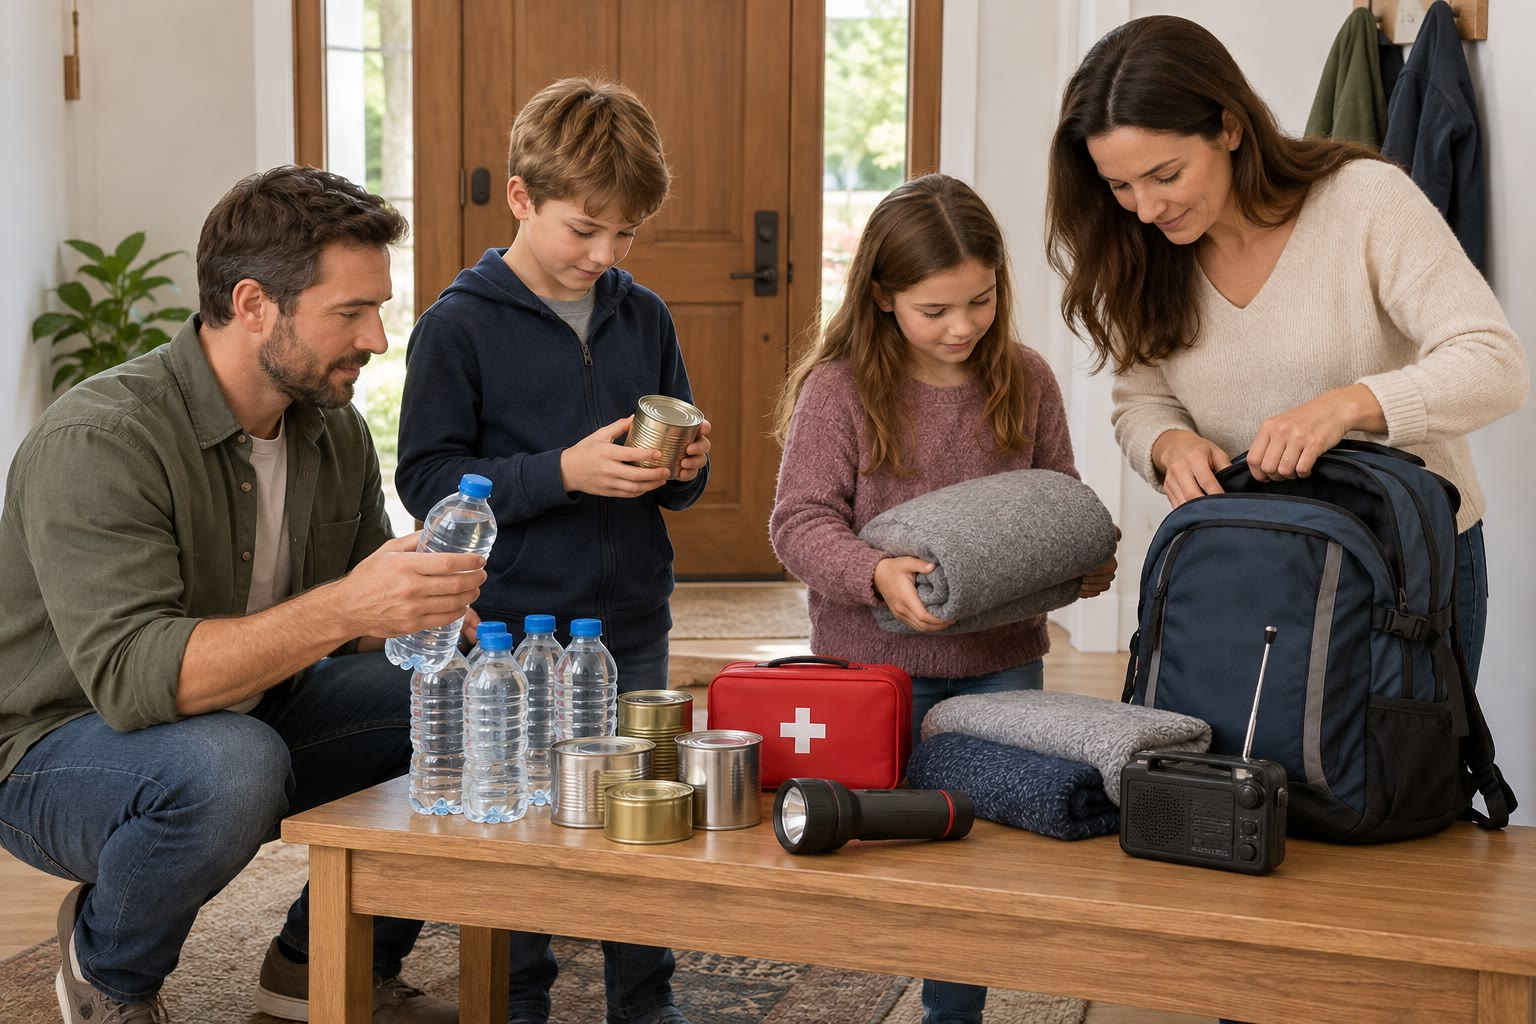
\includegraphics[width=\linewidth]{images/book1/ai/g9-emergency-kit.jpg}
\end{minipage}\hfill
\begin{minipage}[c]{0.52\linewidth}\raggedright
{\small Estar preparados: una familia revisa su kit de emergencia,
guardado cerca de la puerta, listo para llevárselo si tiene que marcharse
deprisa: agua y comida que se conserve varios días, una linterna, una radio
que funcione sin la red eléctrica, pilas de repuesto, un botiquín y mantas
de abrigo (ilustración generada por IA de una escena genérica).}
\end{minipage}
% ledger: ready:kit
\label{fig:g9:natural-risks:kit}
\end{omfigure}

\section{Vigilar los volcanes y las fallas}

Un observatorio vulcanológico vigila las señales de alerta del
\cref{ch:g7:volcanoes} con instrumentos que funcionan día y noche y envían
sus lecturas al observatorio.
% ledger: usgs:hvo-toolkit

\begin{omfigure}
\begin{tikzpicture}[x=1cm, y=1cm, font=\footnotesize, >={Stealth[length=2mm]}]
  % ground and cone
  \fill[black!13] (0,0) -- (0,1.0) -- (3.0,1.2) -- (5.4,3.6) -- (6.4,3.6) -- (8.8,1.2) -- (12,1.0) -- (12,0) -- cycle;
  \draw[black!60] (0,1.0) -- (3.0,1.2) -- (5.4,3.6) -- (6.4,3.6) -- (8.8,1.2) -- (12,1.0);
  % magma chamber and conduit
  \fill[omWarm!70] (5.9,0.6) ellipse (1.5 and 0.38);
  \fill[omWarm!70] (5.75,0.9) rectangle (6.05,3.6);
  \node[white, font=\scriptsize\bfseries] at (5.9,0.58) {magma};
  % gas plume, drifting west
  \fill[black!10] (5.8,3.95) circle (0.3) (5.35,4.35) circle (0.4) (4.75,4.75) circle (0.45);
  % swollen east flank, dashed
  \draw[dashed, omWarm, line width=0.8pt] (6.45,3.7) .. controls (7.5,3.55) and (8.6,2.6) .. (8.85,1.25);
  \draw[->, omWarm] (7.3,2.75) -- (7.7,3.15);
  \node[anchor=west, align=left, text=omWarm!80!black] at (8.2,3.75) {el magma que sube\\ hincha la ladera};
  % tiltmeter on the east flank
  \fill[black] (7.75,2.12) rectangle (8.05,2.24);
  \draw[black!70] (8.1,2.2) -- (8.5,2.45);
  \node[anchor=west, align=left] at (8.5,2.55) {inclinómetro: la ladera\\ se inclina al hincharse};
  % GPS receiver on the west flank, and its satellite
  \draw[black, line width=0.6pt] (4.4,2.6) -- (4.4,2.95);
  \fill[black] (4.25,2.95) rectangle (4.55,3.05);
  \draw[black] (4.4,3.05) circle (0.1);
  \draw[black, fill=white] (1.7,4.85) rectangle (2.0,5.05);
  \draw[black] (1.4,4.95) -- (2.3,4.95);
  \node[anchor=east] at (1.35,4.95) {satélite};
  \draw[black!50, dashed] (4.3,3.15) -- (2.05,4.8);
  \draw[black!70] (3.05,2.65) -- (4.2,2.85);
  \node[anchor=east, align=right] at (3.0,2.6) {receptor GPS: el\\ suelo se mueve\\ unos milímetros};
  % gas instrument on the crater rim
  \fill[black] (6.45,3.6) rectangle (6.75,3.75);
  \draw[black!70] (6.8,3.75) -- (7.1,4.45);
  \node[anchor=west, align=left] at (7.1,4.6) {instrumento de gases: los gases\\ que escapan del cráter};
  % seismometer (in the ground)
  \fill[black] (2.1,0.95) rectangle (2.4,1.1);
  \node[anchor=north, align=center] at (1.6,0.85) {sismómetro:\\ pequeños terremotos};
  % camera, east, looking at the summit
  \fill[black] (10.7,1.12) rectangle (11.0,1.32);
  \fill[black] (10.7,1.17) -- (10.55,1.12) -- (10.55,1.32) -- (10.7,1.27) -- cycle;
  \node[anchor=north, align=center] at (10.8,0.85) {cámara:\\ vigila la cima};
\end{tikzpicture}

{\small Vigilar un \omterm{def:g4:volcanoes-earthquakes-first-look:volcano}{volcán} (un esquema, no a escala). Los \omterm{def:g7:earthquakes:seismometer}{sismómetros}
cuentan los pequeños \omterm{def:g4:volcanoes-earthquakes-first-look:earthquake}{terremotos}; los inclinómetros y los receptores GPS,
fijados a la \omterm{def:g3:stones-pebbles-sand:rock}{roca}, miden cómo se inclina y se desplaza el suelo a medida
que el \omterm{def:g7:volcanoes:magma}{magma} se acumula debajo; otros instrumentos miden los gases que
escapan; las cámaras vigilan la cima. Los \omterm{def:g4:clouds-rain-snow:rain-gauge}{pluviómetros} ayudan a distinguir
las señales del \omterm{def:g4:volcanoes-earthquakes-first-look:volcano}{volcán} de los efectos de las \omterm{def:g4:clouds-rain-snow:precipitation}{lluvias} intensas.}
% ledger: usgs:hvo-toolkit
\label{fig:g9:natural-risks:monitoring}
\end{omfigure}

Ninguna de estas señales da el día y la hora de una \omterm{def:g4:volcanoes-earthquakes-first-look:eruption}{erupción}. Los
científicos las leen juntas, como un médico lee varias medidas de un
paciente, y dicen cómo cambia el peligro; las autoridades deciden cuándo
cerrar una zona y cuándo evacuar a la población. En el Pinatubo, esta
cadena funcionó. En el Nevado del Ruiz, el \omterm{def:g4:volcanoes-earthquakes-first-look:volcano}{volcán} llevaba un año dando
señales, con enjambres de \omterm{def:g4:volcanoes-earthquakes-first-look:earthquake}{terremotos}, pero los instrumentos eran pocos, y
la cadena que iba de los científicos a los habitantes de Armero estaba
rota.
% ledger: usgs:armero, usgs:hvo-toolkit, usgs:pinatubo-1991

Las \omterm{def:g7:earthquakes:fault}{fallas} se vigilan de la misma manera, con redes de \omterm{def:g7:earthquakes:seismometer}{sismómetros} y de
estaciones GPS que miden, milímetro a milímetro, cómo se desplazan
lentamente los dos lados de una \omterm{def:g7:earthquakes:fault}{falla}. Así se sabe qué \omterm{def:g7:earthquakes:fault}{fallas} están
acumulando la tensión del próximo gran \omterm{def:g4:volcanoes-earthquakes-first-look:earthquake}{terremoto}, pero no cuándo llegará.
Frente a los \omterm{def:g4:volcanoes-earthquakes-first-look:earthquake}{terremotos}, la \omterm{def:g9:natural-risks:prevention}{prevención} es la principal defensa.
% ledger: usgs:gps, usgs:eq-basics

\section{Mapas de peligrosidad y zonas inundables}

El primer paso de la \omterm{def:g9:natural-risks:prevention}{prevención} es saber dónde puede golpear un peligro.

\begin{definition}[Mapa de peligrosidad]\label{def:g9:natural-risks:hazard-map}
Un \emph{mapa de peligrosidad}\index{mapa de peligrosidad} muestra los
lugares que puede alcanzar un \omterm{def:g5:natural-hazards:hazard}{peligro natural}, a menudo con varios niveles
de peligro. Se elabora a partir de lo que el peligro ha hecho en el pasado
y de la forma del terreno.
\end{definition}

El \omterm{def:g2:drawing-to-map:map}{mapa} del Nevado del Ruiz, al principio de este capítulo, es un \omterm{def:g9:natural-risks:hazard-map}{mapa de
peligrosidad}: las coladas de \omterm{def:g3:stones-pebbles-sand:sand}{barro} del pasado habían seguido los \omterm{def:g1:landscapes-around-us:landform}{valles}, y
las siguientes los seguirían también. Los \omterm{def:g2:drawing-to-map:map}{mapas} de \omterm{def:g5:water-shapes-the-land:flood}{inundación} siguen la
misma idea. El agua se extiende por el terreno bajo y llano que bordea un
\omterm{def:g1:landscapes-around-us:water}{río}: cuanto más alta es la \omterm{def:g5:water-shapes-the-land:flood}{crecida}, más ancha es la franja de terreno que
cubre. Un \omterm{def:g2:drawing-to-map:map}{mapa} de \omterm{def:g5:water-shapes-the-land:flood}{inundación} traza el borde del agua para una \omterm{def:g5:water-shapes-the-land:flood}{crecida}
elegida, a menudo la que tiene una probabilidad de 1 entre 100 de ser
alcanzada o superada en un año cualquiera. Se la llama \emph{\omterm{def:g5:water-shapes-the-land:flood}{crecida} de
cien años}, pero no es una \omterm{def:g5:water-shapes-the-land:flood}{crecida} que llegue una vez por siglo: puede
llegar dos años seguidos.
% ledger: fema:flood-zones

\begin{omfigure}
\begin{tikzpicture}
\begin{axis}[axis equal image, xmin=3.5, xmax=7, ymin=2.7, ymax=5.5, width=11.5cm,
  enlargelimits=false, tick label style={font=\scriptsize}, xlabel={este (km)},
  ylabel={norte (km)}, label style={font=\small}, xtick={3.5,4,...,7}, ytick={3,3.5,...,5.5},
  clip mode=individual]
\addplot[contour] table {figdata/out/grade-9-flood_zone-contours.dat};
\addplot[index contour] table {figdata/out/grade-9-flood_zone-index.dat};
\addplot[fill=omSea, draw=blue!40, line width=0.3pt] table {figdata/out/grade-9-flood_zone-zone10.dat} -- cycle;
\addplot[fill=blue!25, draw=blue!50, line width=0.3pt] table {figdata/out/grade-9-flood_zone-zone.dat} -- cycle;
\addplot[fill=blue!50, draw=none] table {figdata/out/grade-9-flood_zone-zone2.dat} -- cycle;
\addplot[only marks, mark=none, point meta=explicit symbolic, nodes near coords,
  nodes near coords align={center}, nodes near coords style={font=\tiny, fill=white, inner sep=0.6pt, text=omContour}]
  table[meta=z] {figdata/out/grade-9-flood_zone-index-lab.dat};
\addplot[river] table {figdata/out/grade-9-flood_zone-river.dat};
\end{axis}
\end{tikzpicture}

\smallskip
\begin{tikzpicture}[font=\footnotesize]
  \node[anchor=east] at (0,0.125) {crecida sobre el nivel del río:};
  \fill[blue!50] (0.2,0) rectangle (0.7,0.25); \node[anchor=west] at (0.8,0.125) {\qty{2}{m}};
  \fill[blue!25, draw=blue!50, line width=0.3pt] (1.9,0) rectangle (2.4,0.25); \node[anchor=west] at (2.5,0.125) {\qty{5}{m}};
  \fill[omSea, draw=blue!40, line width=0.3pt] (3.6,0) rectangle (4.1,0.25); \node[anchor=west] at (4.2,0.125) {\qty{10}{m}};
\end{tikzpicture}

{\small La \omterm{def:g5:water-shapes-the-land:flood}{llanura de inundación} del \omterm{def:g1:landscapes-around-us:water}{río} de las Colinas de Varden, que
fluye hacia el este. Cada tono es el terreno que cubriría una \omterm{def:g5:water-shapes-the-land:flood}{crecida} que
subiera 2, 5 o \qty{10}{m} por encima del nivel normal del \omterm{def:g1:landscapes-around-us:water}{río}: cada zona
contiene a las más pequeñas. Las zonas son estrechas porque las laderas del
\omterm{def:g1:landscapes-around-us:landform}{valle} se elevan deprisa desde su fondo llano. Las líneas finas unen puntos
de la misma \omterm{def:g4:world-physical-map:altitude}{altitud}, cada \qty{10}{m}, rotuladas cada \qty{50}{m}; estos
\omterm{def:g2:drawing-to-map:map}{mapas} son el tema del \cref{ch:g9:maps-of-the-earth}.}
% ledger: (invented region: figdata/grade-9/flood_zone.py, parts zone2, zone, zone10)
\label{fig:g9:natural-risks:flood-zones}
\end{omfigure}

\begin{method}[Leer un mapa de zonas inundables]
\begin{enumerate}
  \item Averigua a qué \omterm{def:g5:water-shapes-the-land:flood}{crecida} corresponde la zona: a qué altura sobre el
        \omterm{def:g1:landscapes-around-us:water}{río}, o con qué frecuencia puede llegar.
  \item Sitúa el lugar en el \omterm{def:g2:drawing-to-map:map}{mapa}, con la \omterm{def:g2:drawing-to-map:scale}{escala} gráfica o la cuadrícula.
  \item Si el lugar está dentro de la zona sombreada, esa \omterm{def:g5:water-shapes-the-land:flood}{crecida} lo
        alcanzaría; si está fuera, quedaría seco en esa \omterm{def:g5:water-shapes-the-land:flood}{crecida}, pero no
        en todas las \omterm{def:g5:water-shapes-the-land:flood}{crecidas}.
  \item Para comparar lugares, usa su altura sobre el \omterm{def:g1:landscapes-around-us:water}{río}: cuanto más
        bajos, más a menudo se inundan.
\end{enumerate}
\end{method}

\begin{example}[Tres casas junto al río]
En un \omterm{def:g2:drawing-to-map:map}{mapa} como el de arriba, una casa se levanta sobre un terreno
situado \qty{3}{m} por encima del \omterm{def:g1:landscapes-around-us:water}{río}. Una \omterm{def:g5:water-shapes-the-land:flood}{crecida} de \qty{2}{m} sobre el
\omterm{def:g1:landscapes-around-us:water}{río} no la alcanza; las de 5 y \qty{10}{m}, sí. Una segunda casa, a
\qty{8}{m} sobre el \omterm{def:g1:landscapes-around-us:water}{río}, solo la alcanza la \omterm{def:g5:water-shapes-the-land:flood}{crecida} de \qty{10}{m}, y una
tercera, en una ladera a \qty{30}{m} sobre el \omterm{def:g1:landscapes-around-us:water}{río}, ninguna de las tres. La
primera casa es la más vulnerable: le bastan \omterm{def:g5:water-shapes-the-land:flood}{crecidas} más pequeñas, que
llegan más a menudo, para alcanzarla.
\end{example}

\section{Construir para resistir los terremotos}

Durante un \omterm{def:g4:volcanoes-earthquakes-first-look:earthquake}{terremoto}, el suelo se mueve de un lado a otro bajo un edificio,
y el edificio se sacude desde abajo; en un \omterm{def:g4:volcanoes-earthquakes-first-look:earthquake}{terremoto} fuerte, el peligro
procede sobre todo de los edificios que se agrietan y se derrumban. Los
ingenieros no pueden detener la sacudida, pero pueden construir de modo
que la estructura soporte las fuerzas de la sacudida sin derrumbarse.
% ledger: iris:better-wall

\begin{omfigure}
\begin{tikzpicture}[x=1cm, y=1cm, font=\footnotesize, >={Stealth[length=2mm]}]
  % panel 1: a frame that leans
  \begin{scope}
    \fill[black!13] (-0.3,-0.25) rectangle (3.0,0);
    \draw[black!35, dashed] (0.2,0) rectangle (2.5,2.6);
    \draw[black, line width=1.2pt] (0.2,0) -- (0.75,2.6) -- (3.05,2.6) -- (2.5,0);
    \draw[black, line width=1.2pt] (0.47,1.3) -- (2.77,1.3);
    \draw[<->] (0.2,-0.45) -- (1.0,-0.45);
    \node[align=center, anchor=north] at (1.35,-0.65) {(a) una estructura sola\\ se inclina y puede caer};
  \end{scope}
  % panel 2: braces
  \begin{scope}[xshift=3.7cm]
    \fill[black!13] (-0.3,-0.25) rectangle (3.0,0);
    \draw[black, line width=1.2pt] (0.2,0) rectangle (2.5,2.6);
    \draw[black, line width=1.2pt] (0.2,1.3) -- (2.5,1.3);
    \draw[omWarm, line width=1pt] (0.2,0) -- (2.5,1.3) (2.5,0) -- (0.2,1.3)
                                  (0.2,1.3) -- (2.5,2.6) (2.5,1.3) -- (0.2,2.6);
    \node[align=center, anchor=north] at (1.35,-0.65) {(b) las riostras diagonales\\ mantienen su forma};
  \end{scope}
  % panel 3: shear wall
  \begin{scope}[xshift=7.4cm]
    \fill[black!13] (-0.3,-0.25) rectangle (3.0,0);
    \draw[black, line width=1.2pt] (0.2,0) rectangle (2.5,2.6);
    \draw[black, line width=1.2pt] (0.2,1.3) -- (2.5,1.3);
    \fill[omWarm!35] (1.6,0) rectangle (2.5,2.6);
    \draw[black, line width=0.6pt] (1.6,0) rectangle (2.5,2.6);
    \node[align=center, anchor=north] at (1.35,-0.65) {(c) un muro de cortante rígido\\ de arriba abajo};
  \end{scope}
  % panel 4: base isolation
  \begin{scope}[xshift=11.1cm]
    \fill[black!13] (-0.3,-0.25) rectangle (3.0,0);
    \foreach \x in {0.35,1.35,2.35} \fill[omSea, draw=black!60, rounded corners=1pt] (\x-0.18,0) rectangle (\x+0.18,0.3);
    \draw[black, line width=1.2pt] (0.15,0.3) -- (2.55,0.3);
    \draw[black, line width=1.2pt] (0.2,0.3) rectangle (2.5,2.7);
    \draw[black, line width=1.2pt] (0.2,1.5) -- (2.5,1.5);
    \draw[<->] (0.2,-0.45) -- (1.0,-0.45);
    \node[align=center, anchor=north] at (1.35,-0.65) {(d) los aisladores dejan\\ que el suelo se mueva debajo};
  \end{scope}
\end{tikzpicture}

{\small Cuatro estructuras sacudidas por el mismo suelo (un esquema). Una
estructura de pilares y vigas sola se inclina y puede derrumbarse (a). Las
riostras diagonales (b) y los muros de cortante rígidos (c) impiden que se
incline; unas uniones sólidas entre las vigas y los pilares la mantienen
unida. Los aisladores colocados bajo el edificio (d) ceden cuando el suelo
se mueve, de modo que al edificio le llega mucho menos movimiento.}
% ledger: iris:better-wall, explo:base-isolation
\label{fig:g9:natural-risks:buildings}
\end{omfigure}

Los mismos principios sirven para una casa, una escuela o un puente. Son
más fáciles de aplicar cuando se diseña el edificio que cuando se añaden
después a un edificio antiguo.

\begin{inthelab}[Una torre sobre una bandeja que se sacude]
En el interior, construye dos torrecitas de la misma altura con pajitas o
palitos de madera y plastilina, en forma de estructuras de dos plantas.
Pon riostras diagonales en todas las caras de la segunda. Coloca las dos
sobre una bandeja y desliza después la bandeja deprisa de un lado a otro,
suavemente al principio y luego con más fuerza. ¿Qué torre se inclina
primero? ¿Cuál mantiene su forma? Coloca después la torre sin riostras
sobre cuatro canicas, bajo una cartulina ligera, y vuelve a sacudir: ¿qué
cambia?
\end{inthelab}

\section{Alertas a tiempo}

La última parte de la \omterm{def:g9:natural-risks:prevention}{prevención} es la alerta. Para los \omterm{def:g7:earthquakes:tsunami}{tsunamis}, empieza
en el fondo del \omterm{def:g2:water-on-earth:ocean}{océano}. En lugares cercanos a donde ya se han originado
\omterm{def:g7:earthquakes:tsunami}{tsunamis} destructivos, un registrador de presión descansa en el fondo del
\omterm{def:g2:water-on-earth:ocean}{mar} y mide cada \qty{15}{s} el peso del agua que tiene encima, lo que da
la altura de la superficie del \omterm{def:g2:water-on-earth:ocean}{mar}. Envía sus lecturas mediante sonido, a
través del agua, a una boya amarrada en la superficie, y la boya las
retransmite por satélite a los centros de alerta de \omterm{def:g7:earthquakes:tsunami}{tsunamis}. Una subida
del \omterm{def:g2:water-on-earth:ocean}{mar} lejos de cualquier \omterm{def:g1:landscapes-around-us:water}{costa} revela un \omterm{def:g7:earthquakes:tsunami}{tsunami} en camino, horas antes
de que llegue a \omterm{def:g1:landscapes-around-us:water}{costas} lejanas.
% ledger: ndbc:dart, nws:tsunami-speed

\begin{omfigure}
\begin{minipage}[c]{0.4\linewidth}\centering
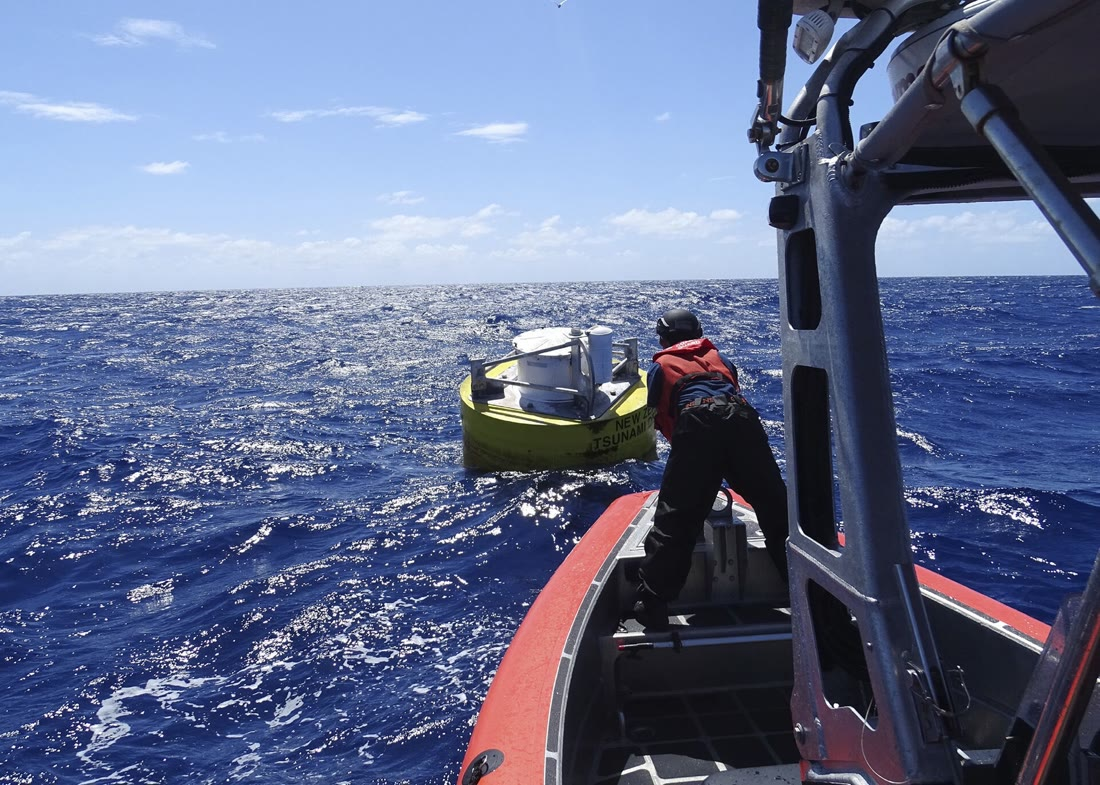
\includegraphics[width=\linewidth]{images/book1/g9-dart-buoy.jpg}
\end{minipage}\hfill
\begin{minipage}[c]{0.56\linewidth}\raggedright
{\small Un tripulante de un buque de la Guardia Costera de Estados Unidos
inspecciona una boya de alerta de \omterm{def:g7:earthquakes:tsunami}{tsunamis} en el \omterm{def:g2:water-on-earth:ocean}{océano} Pacífico, en
noviembre de 2021. La boya flota sobre un registrador de presión situado
en el fondo del \omterm{def:g2:water-on-earth:ocean}{mar}, miles de metros más abajo. U.S. Coast Guard (dominio
público, vía Wikimedia Commons).}
\end{minipage}
% ledger: commons:dart-buoy
\label{fig:g9:natural-risks:buoy}
\end{omfigure}

\begin{history}[Una red de boyas]
En 2001 se completó la primera red de seis estaciones de este tipo, en el
\omterm{def:g2:water-on-earth:ocean}{océano} Pacífico. Después del \omterm{def:g7:earthquakes:tsunami}{tsunami} de diciembre de 2004, que llegó a las
\omterm{def:g1:landscapes-around-us:water}{costas} del \omterm{def:g2:water-on-earth:ocean}{océano} Índico sin que hubiera ningún sistema de alerta
(\cref{ch:g7:earthquakes}), la red creció: en marzo de 2008 había 39
estaciones.
\end{history}
% ledger: ndbc:dart

Una alerta solo salva vidas si llega a personas que saben qué hacer con
ella: las rutas hacia terrenos más altos están señalizadas y se han
practicado, el kit de emergencia está listo, las escuelas hacen
simulacros. En Armero, el peligro se conocía y el \omterm{def:g2:drawing-to-map:map}{mapa} estaba hecho; la
alerta nunca llegó a la ciudad.
% ledger: ready:kit, usgs:armero

\section{Ejercicios}

\begin{exercise}[$\star$]\label{exo:g9:natural-risks:1}
¿Peligro o \omterm{def:g9:natural-risks:vulnerability}{vulnerabilidad}? (a) Un \omterm{def:g1:landscapes-around-us:water}{río} que se desborda casi todas las
primaveras. (b) Un pueblo sin sistema de alerta. (c) Casas pesadas de
ladrillo sin estructura. (d) Un fuerte \omterm{def:g4:volcanoes-earthquakes-first-look:earthquake}{terremoto} en una \omterm{def:g7:earthquakes:fault}{falla} cercana.
(e) Una ciudad construida a la salida de un \omterm{def:g1:landscapes-around-us:landform}{valle} por el que ya han bajado
coladas de \omterm{def:g3:stones-pebbles-sand:sand}{barro}.
\end{exercise}

\begin{exercise}[$\star$]\label{exo:g9:natural-risks:2}
¿Verdadero o falso? Corrige las frases falsas. (a) Un \omterm{def:g5:natural-hazards:hazard}{peligro natural} en
un lugar donde no vive nadie es un \omterm{def:g9:natural-risks:risk}{riesgo} alto. (b) La \omterm{def:g9:natural-risks:prevention}{prevención} puede
reducir la \omterm{def:g9:natural-risks:vulnerability}{vulnerabilidad} de una ciudad. (c) Un \omterm{def:g9:natural-risks:hazard-map}{mapa de peligrosidad}
muestra dónde puede golpear un peligro. (d) Un buen sistema de alerta hace
que un \omterm{def:g4:volcanoes-earthquakes-first-look:volcano}{volcán} sea menos peligroso.
\end{exercise}

\begin{exercise}[$\star$]\label{exo:g9:natural-risks:3}
Para cada peligro, di si se puede prever con días u horas de antelación:
(a) una \omterm{def:g5:natural-hazards:storm}{tormenta}; (b) una \omterm{def:g5:water-shapes-the-land:flood}{inundación} tras \omterm{def:g4:clouds-rain-snow:precipitation}{lluvias} intensas; (c) un
\omterm{def:g4:volcanoes-earthquakes-first-look:earthquake}{terremoto}; (d) la llegada de un \omterm{def:g7:earthquakes:tsunami}{tsunami} a una \omterm{def:g1:landscapes-around-us:water}{costa} lejana del lugar donde
se originó.
\end{exercise}

\begin{exercise}[$\star$]\label{exo:g9:natural-risks:4}
% ledger: usgs:hvo-toolkit
Usa el dibujo de un \omterm{def:g4:volcanoes-earthquakes-first-look:volcano}{volcán} vigilado. ¿Qué mide cada instrumento, y qué
señal de alerta de una \omterm{def:g4:volcanoes-earthquakes-first-look:eruption}{erupción} vigila? (a) Un \omterm{def:g7:earthquakes:seismometer}{sismómetro}. (b) Un
inclinómetro. (c) Un receptor GPS. (d) Un instrumento de gases.
\end{exercise}

\begin{exercise}[$\star\star$]\label{exo:g9:natural-risks:5}
% ledger: usgs:armero
En 1985, las coladas de \omterm{def:g3:stones-pebbles-sand:sand}{barro} del Nevado del Ruiz llegaron a Armero, a
\qty{45}{km}, unas dos horas después de la \omterm{def:g4:volcanoes-earthquakes-first-look:eruption}{erupción}. (a) ¿Cuál fue su
velocidad media, en kilómetros por hora? (b) Una persona camina a unos
\qty{4}{km/h}. ¿Qué distancia habrían podido recorrer a pie los
habitantes en dos horas? (c) ¿Por qué no se marcharon? (d) Da dos cosas
que podrían haberlos salvado.
\end{exercise}

\begin{exercise}[$\star\star$]\label{exo:g9:natural-risks:6}
% ledger: (invented region: figdata/grade-9/flood_zone.py)
Usa el \omterm{def:g2:drawing-to-map:map}{mapa} de \omterm{def:g5:water-shapes-the-land:flood}{zonas inundables} de las Colinas de Varden. (a) ¿Qué \omterm{def:g5:water-shapes-the-land:flood}{crecida}
cubre la franja más ancha? (b) Con la cuadrícula del \omterm{def:g2:drawing-to-map:map}{mapa}, mide la anchura
de cada zona a través del \omterm{def:g1:landscapes-around-us:landform}{valle} a \qty{5}{km} al este. (c) Un granero se
levanta sobre un terreno situado \qty{6}{m} por encima del \omterm{def:g1:landscapes-around-us:water}{río}. ¿Cuáles de
las tres \omterm{def:g5:water-shapes-the-land:flood}{crecidas} lo alcanzan? (d) ¿Por qué la \omterm{def:g5:water-shapes-the-land:flood}{crecida} de \qty{2}{m} sobre
el \omterm{def:g1:landscapes-around-us:water}{río} es la que llega más a menudo?
\end{exercise}

\begin{exercise}[$\star\star$]\label{exo:g9:natural-risks:7}
Sitúa cada situación en la cuadrícula del \omterm{def:g9:natural-risks:risk}{riesgo} (peligro bajo o alto,
\omterm{def:g9:natural-risks:vulnerability}{vulnerabilidad} baja o alta) y di si el \omterm{def:g9:natural-risks:risk}{riesgo} es bajo, moderado o alto.
(a) Edificios sólidos y simulacros en una ciudad sobre una \omterm{def:g7:earthquakes:fault}{falla} activa.
(b) Un camping en la \omterm{def:g5:water-shapes-the-land:flood}{llanura de inundación} de un \omterm{def:g1:landscapes-around-us:water}{río} que rara vez se
desborda. (c) Un pueblo de casas débiles al pie de un \omterm{def:g4:volcanoes-earthquakes-first-look:volcano}{volcán} activo, sin
observatorio. (d) Una ciudad en lo alto de una \omterm{def:g1:landscapes-around-us:landform}{colina}, lejos de cualquier
\omterm{def:g7:earthquakes:fault}{falla}, \omterm{def:g1:landscapes-around-us:water}{río} o \omterm{def:g4:volcanoes-earthquakes-first-look:volcano}{volcán}.
\end{exercise}

\begin{exercise}[$\star\star$]\label{exo:g9:natural-risks:8}
% ledger: iris:better-wall, explo:base-isolation
Se construyen tres escuelas sobre el mismo terreno. La escuela A es una
estructura de pilares y vigas con muros de ladrillo entre ellos; la
escuela B tiene la misma estructura con riostras diagonales y dos muros de
cortante; la escuela C tiene la estructura de B, apoyada sobre aisladores.
(a) Ordénalas de la más segura a la menos segura ante un \omterm{def:g4:volcanoes-earthquakes-first-look:earthquake}{terremoto}.
(b) Explica qué hacen las riostras. (c) Explica qué hacen los aisladores.
\end{exercise}

\begin{exercise}[$\star\star$]\label{exo:g9:natural-risks:9}
% ledger: fema:flood-zones
Un \omterm{def:g2:drawing-to-map:map}{mapa} de \omterm{def:g5:water-shapes-the-land:flood}{inundación} muestra la \omterm{def:g5:water-shapes-the-land:flood}{crecida} de cien años, que tiene una
probabilidad de 1 entre 100 de ser alcanzada o superada en un año
cualquiera. (a) Escribe esta probabilidad como porcentaje. (b) Un vecino
dice: ``La \omterm{def:g5:water-shapes-the-land:flood}{crecida} de cien años llegó el año pasado, así que estamos a
salvo durante 99 años''. ¿Qué falla? (c) Por término medio, ¿cuántas
\omterm{def:g5:water-shapes-the-land:flood}{crecidas} así llegarían en 300 años?
\end{exercise}

\begin{exercise}[$\star\star$]\label{exo:g9:natural-risks:10}
% ledger: ndbc:dart, nws:tsunami-speed
Una estación de alerta de \omterm{def:g7:earthquakes:tsunami}{tsunamis} mide la presión en el fondo del \omterm{def:g2:water-on-earth:ocean}{mar}
cada \qty{15}{s}. (a) ¿Cuántas lecturas hace en una hora? (b) ¿Y en un año
de 365 días? Escribe la respuesta en notación científica. (c) Un \omterm{def:g7:earthquakes:tsunami}{tsunami}
cruza el \omterm{def:g2:water-on-earth:ocean}{océano} profundo a unos \qty{800}{km/h}. ¿Cuánto tarda en llegar a
una \omterm{def:g1:landscapes-around-us:water}{costa} situada a \qty{2400}{km}? (d) ¿Por qué importa ese tiempo?
\end{exercise}

\begin{exercise}[$\star\star\star$]\label{exo:g9:natural-risks:11}
% ledger: ready:kit
Una familia de cuatro personas prepara un kit de emergencia con agua para
3 días, a razón de unos \qty{3.8}{L} por persona y por día, para beber y
lavarse. (a) ¿Cuántos litros de agua necesitan? (b) ¿Cuántas botellas de
\qty{1.5}{L} son? (c) Nombra otras cuatro cosas que contiene el kit, y di
para qué sirve cada una. (d) ¿Por qué se guarda el kit cerca de la puerta?
\end{exercise}

\begin{exercise}[$\star\star\star$]\label{exo:g9:natural-risks:12}
% ledger: usgs:armero, usgs:hvo-toolkit
Una ciudad se encuentra junto a un \omterm{def:g1:landscapes-around-us:water}{río}, a la salida de un \omterm{def:g1:landscapes-around-us:landform}{valle} que baja
de un \omterm{def:g4:volcanoes-earthquakes-first-look:volcano}{volcán} nevado. Bajo sus calles hay depósitos de antiguas coladas de
\omterm{def:g3:stones-pebbles-sand:sand}{barro}. El \omterm{def:g4:volcanoes-earthquakes-first-look:volcano}{volcán} ha empezado a temblar con pequeños \omterm{def:g4:volcanoes-earthquakes-first-look:earthquake}{terremotos}. Redacta un
plan de \omterm{def:g9:natural-risks:prevention}{prevención} de cinco puntos para la ciudad. Para cada punto, di si
actúa sobre el lado del peligro (conocer y vigilar el peligro) o sobre el
lado de la \omterm{def:g9:natural-risks:vulnerability}{vulnerabilidad} del \omterm{def:g9:natural-risks:risk}{riesgo}.
\end{exercise}

\section{Problema: ¿dónde construir la nueva escuela?}

\begin{problem}[{Problema de fin de semana --- se sitúa una nueva escuela en
el mapa de las Colinas de Varden, lejos de las inundaciones, de las
pendientes fuertes y de la falla; la respuesta final es el número de casas
situadas dentro de la zona inundable}]
\label{pb:g9:natural-risks:1}
% ledger: (invented region: figdata/grade-9/flood_zone.py: sites A, B, C; 17 of 28 houses in the 5 m zone)
El pueblo de las Colinas de Varden necesita una nueva escuela, y se
proponen tres emplazamientos: A, B y C, en el \omterm{def:g2:drawing-to-map:map}{mapa} de abajo. La \omterm{def:g5:water-shapes-the-land:flood}{zona
inundable} sombreada en el \omterm{def:g2:drawing-to-map:map}{mapa} es todo el terreno situado a menos de
\qty{5}{m} por encima del \omterm{def:g1:landscapes-around-us:water}{río}, que una gran \omterm{def:g5:water-shapes-the-land:flood}{crecida} cubriría. La tabla da,
para cada emplazamiento, la \omterm{def:g4:world-physical-map:altitude}{altitud} del terreno, el nivel del \omterm{def:g1:landscapes-around-us:water}{río} a su
lado y cuánto se eleva el terreno a lo largo de \qty{200}{m} medidos en
horizontal a través de la ladera.

\begin{center}
{\small
\begin{tabular}{|c|c|c|c|}
\hline
emplazamiento & \omterm{def:g4:world-physical-map:altitude}{altitud} del terreno & nivel del \omterm{def:g1:landscapes-around-us:water}{río} a su lado & elevación del terreno en \qty{200}{m} \\
\hline
A & \qty{137}{m} & \qty{137}{m} & \qty{1.4}{m} \\
B & \qty{276}{m} & \qty{126}{m} & \qty{83}{m} \\
C & \qty{236}{m} & \qty{143}{m} & \qty{20}{m} \\
\hline
\end{tabular}}
\end{center}

\begin{omfigure}
\begin{tikzpicture}
\begin{axis}[axis equal image, xmin=3.5, xmax=7, ymin=2.7, ymax=5.5, width=11.5cm,
  enlargelimits=false, tick label style={font=\scriptsize}, xlabel={este (km)},
  ylabel={norte (km)}, label style={font=\small}, xtick={3.5,4,...,7}, ytick={3,3.5,...,5.5}]
\addplot[contour] table {figdata/out/grade-9-flood_zone-contours.dat};
\addplot[index contour] table {figdata/out/grade-9-flood_zone-index.dat};
\addplot[fill=blue!25, draw=blue!50, line width=0.3pt] table {figdata/out/grade-9-flood_zone-zone.dat} -- cycle;
\addplot[only marks, mark=none, point meta=explicit symbolic, nodes near coords,
  nodes near coords align={center}, nodes near coords style={font=\tiny, fill=white, inner sep=0.6pt, text=omContour}]
  table[meta=z] {figdata/out/grade-9-flood_zone-index-lab.dat};
\addplot[river] table {figdata/out/grade-9-flood_zone-river.dat};
\addplot[fault] table {figdata/out/shared-region-fault.dat};
\addplot[only marks, mark=square*, mark size=1.5pt, mark options={fill=black}] table {figdata/out/grade-9-flood_zone-houses-in.dat};
\addplot[only marks, mark=square*, mark size=1.5pt, mark options={fill=black}] table {figdata/out/grade-9-flood_zone-houses-out.dat};
\addplot[only marks, mark=*, mark size=2.6pt, mark options={fill=omWarm, draw=black}, point meta=explicit symbolic,
  nodes near coords, nodes near coords align={anchor=south west},
  nodes near coords style={font=\small\bfseries, fill=white, inner sep=1pt, xshift=2.5pt, yshift=2.5pt}]
  table[meta=name] {figdata/out/grade-9-flood_zone-sites.dat};
\node[font=\footnotesize, fill=white, inner sep=1pt, anchor=west] at (axis cs:6.42,5.05) {falla};
\coordinate (na) at (axis cs:3.7,4.75);
\fill[black] (axis cs:5.8,2.85) rectangle (axis cs:5.925,2.9);
\fill[white] (axis cs:5.925,2.85) rectangle (axis cs:6.05,2.9);
\fill[black] (axis cs:6.05,2.85) rectangle (axis cs:6.175,2.9);
\fill[white] (axis cs:6.175,2.85) rectangle (axis cs:6.3,2.9);
\draw[black, line width=0.4pt] (axis cs:5.8,2.85) rectangle (axis cs:6.3,2.9);
\node[font=\footnotesize, above, inner sep=1.5pt, fill=white] at (axis cs:6.05,2.9) {\qty{500}{m}};
\end{axis}
\fill[white, opacity=0.85] ($(na)+(-0.35,-0.1)$) rectangle ($(na)+(0.35,1.45)$);
\pic at (na) {northarrow};
\end{tikzpicture}

{\small El pueblo, los tres emplazamientos para la escuela y la \omterm{def:g5:water-shapes-the-land:flood}{zona
inundable} (sombreada), en el \omterm{def:g2:drawing-to-map:map}{mapa} de las Colinas de Varden (líneas finas
de igual \omterm{def:g4:world-physical-map:altitude}{altitud} cada \qty{10}{m}). Cada cuadradito negro es una casa. La
línea negra gruesa es una \omterm{def:g7:earthquakes:fault}{falla}.}
\label{fig:g9:natural-risks:school-map}
\end{omfigure}

\noindent\textbf{Parte I --- La zona inundable.}\par\nopagebreak
\begin{enumerate}[beginpenalty=10000]
  \item Con los niveles del \omterm{def:g1:landscapes-around-us:water}{río} de la tabla, di en qué sentido fluye el
        \omterm{def:g1:landscapes-around-us:water}{río}.
  \item Calcula la altura de cada emplazamiento sobre el \omterm{def:g1:landscapes-around-us:water}{río} a su lado.
  \item ¿Cuál de los tres emplazamientos está en la \omterm{def:g5:water-shapes-the-land:flood}{zona inundable}?
  \item Usa la \omterm{def:g2:drawing-to-map:scale}{escala} gráfica para medir la anchura de la \omterm{def:g5:water-shapes-the-land:flood}{zona inundable},
        a través del \omterm{def:g1:landscapes-around-us:landform}{valle}, en el emplazamiento A.
\end{enumerate}

\noindent\textbf{Parte II --- Las pendientes y la falla.}\par\nopagebreak
\begin{enumerate}[resume, beginpenalty=10000]
  \item Una pendiente en tanto por ciento es la elevación del terreno por
        cada \qty{100}{m} medidos en horizontal. Calcula la pendiente en
        cada emplazamiento.
  \item ¿Qué emplazamiento estaría expuesto a un \omterm{def:g5:natural-hazards:landslide}{deslizamiento de tierra}?
        Explícalo.
  \item Usa la \omterm{def:g2:drawing-to-map:scale}{escala} gráfica para estimar la distancia de cada
        emplazamiento a la \omterm{def:g7:earthquakes:fault}{falla}.
  \item Supón que la \omterm{def:g7:earthquakes:fault}{falla} todavía puede moverse. ¿Por qué el terreno
        situado justo encima de ella es un mal lugar para una escuela?
\end{enumerate}

\noindent\textbf{Parte III --- Elegir.}\par\nopagebreak
\begin{enumerate}[resume, beginpenalty=10000]
  \item Dibuja una tabla con una fila por emplazamiento y tres columnas:
        ¿en la \omterm{def:g5:water-shapes-the-land:flood}{zona inundable}? ¿pendiente fuerte? ¿sobre la \omterm{def:g7:earthquakes:fault}{falla}?
        Rellénala con sí o no.
  \item ¿Qué emplazamiento elegirías? Justifica tu elección con la tabla.
  \item El emplazamiento elegido sigue estando en una región donde el
        suelo puede temblar. Nombra dos maneras de construir la escuela, y
        un hábito de sus alumnos, que reduzcan su \omterm{def:g9:natural-risks:vulnerability}{vulnerabilidad}.
  \item La escuela servirá también de refugio durante las \omterm{def:g5:water-shapes-the-land:flood}{inundaciones}.
        Cuenta las casas del pueblo que están dentro de la \omterm{def:g5:water-shapes-the-land:flood}{zona inundable}.
        ¿Qué fracción del total de casas representan?
\end{enumerate}
\end{problem}
